% Options for packages loaded elsewhere
\PassOptionsToPackage{unicode}{hyperref}
\PassOptionsToPackage{hyphens}{url}
%
\documentclass[
]{article}
\title{Themelio Yellow Paper v1}
\author{}
\date{2018-12-29T11:02:05+06:00}

\usepackage{amsmath,amssymb}
\usepackage{lmodern}
\usepackage{iftex}
\ifPDFTeX
  \usepackage[T1]{fontenc}
  \usepackage[utf8]{inputenc}
  \usepackage{textcomp} % provide euro and other symbols
\else % if luatex or xetex
  \usepackage{unicode-math}
  \defaultfontfeatures{Scale=MatchLowercase}
  \defaultfontfeatures[\rmfamily]{Ligatures=TeX,Scale=1}
\fi
% Use upquote if available, for straight quotes in verbatim environments
\IfFileExists{upquote.sty}{\usepackage{upquote}}{}
\IfFileExists{microtype.sty}{% use microtype if available
  \usepackage[]{microtype}
  \UseMicrotypeSet[protrusion]{basicmath} % disable protrusion for tt fonts
}{}
\makeatletter
\@ifundefined{KOMAClassName}{% if non-KOMA class
  \IfFileExists{parskip.sty}{%
    \usepackage{parskip}
  }{% else
    \setlength{\parindent}{0pt}
    \setlength{\parskip}{6pt plus 2pt minus 1pt}}
}{% if KOMA class
  \KOMAoptions{parskip=half}}
\makeatother
\usepackage{xcolor}
\IfFileExists{xurl.sty}{\usepackage{xurl}}{} % add URL line breaks if available
\IfFileExists{bookmark.sty}{\usepackage{bookmark}}{\usepackage{hyperref}}
\hypersetup{
  pdftitle={Themelio Yellow Paper v1},
  hidelinks,
  pdfcreator={LaTeX via pandoc}}
\urlstyle{same} % disable monospaced font for URLs
\usepackage{listings}
\newcommand{\passthrough}[1]{#1}
\lstset{defaultdialect=[5.3]Lua}
\lstset{defaultdialect=[x86masm]Assembler}
\usepackage{graphicx}
\makeatletter
\def\maxwidth{\ifdim\Gin@nat@width>\linewidth\linewidth\else\Gin@nat@width\fi}
\def\maxheight{\ifdim\Gin@nat@height>\textheight\textheight\else\Gin@nat@height\fi}
\makeatother
% Scale images if necessary, so that they will not overflow the page
% margins by default, and it is still possible to overwrite the defaults
% using explicit options in \includegraphics[width, height, ...]{}
\setkeys{Gin}{width=\maxwidth,height=\maxheight,keepaspectratio}
% Set default figure placement to htbp
\makeatletter
\def\fps@figure{htbp}
\makeatother
\setlength{\emergencystretch}{3em} % prevent overfull lines
\providecommand{\tightlist}{%
  \setlength{\itemsep}{0pt}\setlength{\parskip}{0pt}}
\setcounter{secnumdepth}{-\maxdimen} % remove section numbering
\ifLuaTeX
  \usepackage{selnolig}  % disable illegal ligatures
\fi

\begin{document}
\maketitle

In this ``yellow paper'', we discuss Themelio's abstract model of the
state of the blockchain. Themelio uses a richly-scripted coin-based
model that is different from both the simple coin-based model of Bitcoin
and the accounts-and-contracts model of Ethereum.

\begin{center}\rule{0.5\linewidth}{0.5pt}\end{center}

\hypertarget{basic-concepts}{%
  \section{Basic concepts}\label{basic-concepts}}

\hypertarget{blockchains-as-state-machines}{%
  \subsection{Blockchains as state
    machines}\label{blockchains-as-state-machines}}

Throughout this yellow paper, we will be discussing Themelio as a
\emph{transaction-based state machine}, a conceptual framework
introduced by the creators of Ethereum in
\href{https://ethereum.github.io/yellowpaper/paper.pdf}{their yellow
  paper}. What this means is that a blockchain starts with a genesis
state, which is mutated by transactions over time, finally ending at the
blockchain at its current state.

\emph{Transactions}, in this model, are arcs between valid states, and
only states that can be reached by repeatedly applying valid
transactions to the genesis state are valid states in the blockchain.
Formally, we can say that

\[\sigma' \equiv \Upsilon(\sigma, T)\]

where \(\Upsilon\) is the state transition function, \(T\) is a
transaction, \(\sigma\) is the state before the transaction entered the
blockchain, and \(\sigma'\) is the state afterwards.

A blockchain, however, does not exactly consist of a linear history of
transactions --- transactions are collated into \emph{blocks}, each of
which can contain a large number of transactions, and possibly auxiliary
data. This collation process then forms a coarse-grained journal of
transactions. A more accurate formalization, then, uses a
\emph{block-level} state transition function \(\Pi\):

\[
  \begin{aligned}
    \sigma_{i+1}  & \equiv \Pi(\sigma_i, B)                                     \newline \\
    B             & \equiv (F, (T_0,T_1,\dots))                      \newline            \\
    \Pi(\sigma,B) & \equiv \Omega(B, \Upsilon(\Upsilon(\sigma, T_0), T_1)\dots)
  \end{aligned}
\]

where \(\Omega\) is the \emph{block sealing function} that assembles a
final state out of the result of applying all the transactions \(T_i\)
within block \(B\), in addition to a \emph{sealing event} \(F\) which
includes per-block actions such as collecting fees.

We believe that treating a blockchain as fundamentally a state machine
is a much more helpful model than simply a series of transactions, even
for coin/UTXO-based blockchains like Themelio. Furthermore, Themelio
extensively uses explicit on-chain representations of the current
blockchain state, rather than making most of the state implicit as in
Bitcoin.

\hypertarget{a-note-on-notation}{%
  \subsubsection{A note on notation}\label{a-note-on-notation}}

We introduced the notion of seeing the blockchain in terms of state
transitions using mathematical notation akin to that used in existing
work such as the Ethereum yellow paper. However, standard mathematical
notation poses an unnecessary obstacle to clarity in two common
situations:

\begin{itemize}
  \tightlist
  \item
        There isn't a reasonable way of representing data with many named
        fields (``structs''). Sets of key-value tuples don't capture the fact
        that a canonical field ordering exists, while straight tuples of
        values force the keys of a struct \(s\) to be the extremely
        inconvenient \(s_1\),\(s_2\),etc
  \item
        When we need to introduce many variables, the mathematical convention
        of using single-letter variables hinders clarity just like code that
        uses single-letter variables. It's often difficult to keep track of a
        bunch of uppercase, lowercase, and Greek letters that aren't shorthand
        for obvious words.
\end{itemize}

Thus, for the remainder of the paper, we will use a ``hybrid'' approach:

\begin{itemize}
  \tightlist
  \item
        Actions will be written in terms of both mathematical functions and
        pseudocode
  \item
        Datatypes will be defined using the Rust programming language
  \item
        Names are often ``codelike'', i.e.~we might name a transaction
        \(\mathsf{foobar}\) rather than \(T_1\).
\end{itemize}

We hope this combines the clarity of ``pseudocode notation'' and the
succinctness of mathematical notation.

\hypertarget{state-transitions-a-glance}{%
  \subsection{State transitions a
    glance}\label{state-transitions-a-glance}}

Let's first take a look at the basic flow of Themelio's state
transitions. As the following picture illustrates, this is based on two
basic datatypes \passthrough{\lstinline!State!} and
\passthrough{\lstinline!SealedState!}. Both of these datatypes will be
described in further detail later.

\begin{figure}
  \centering
  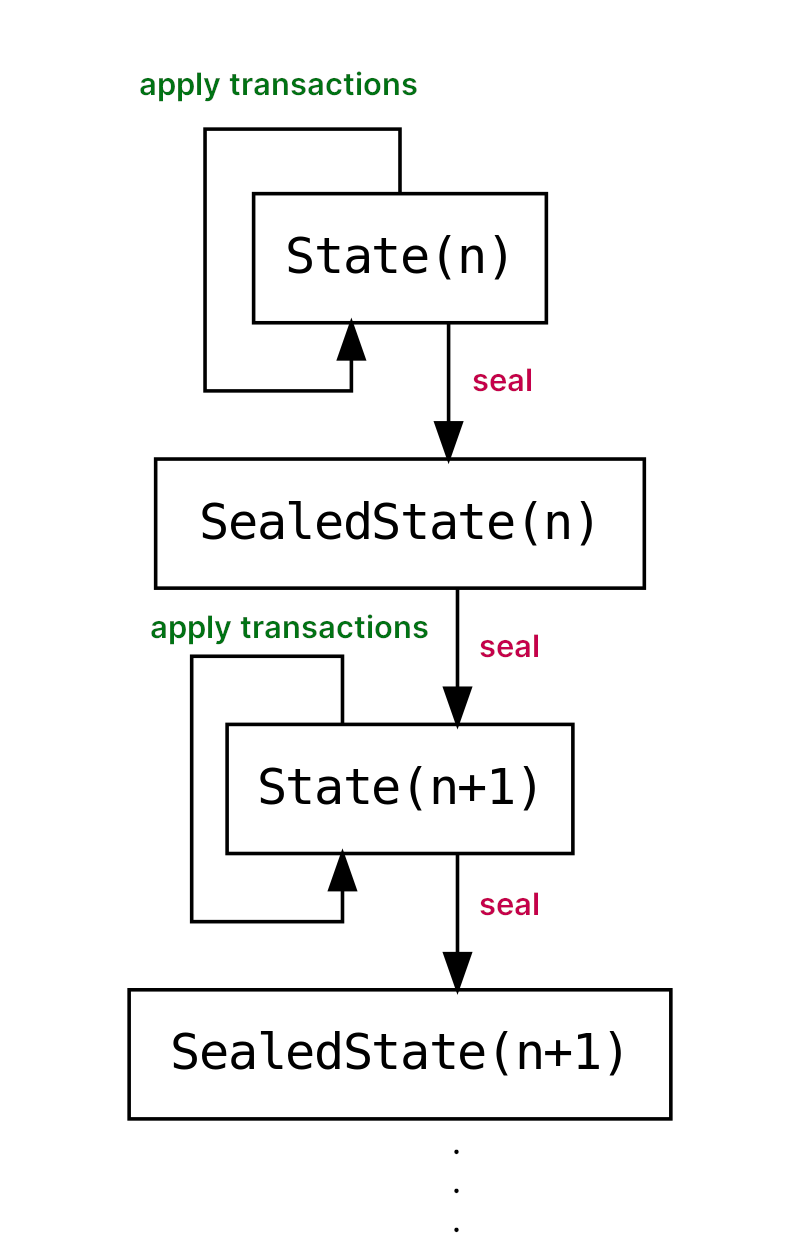
\includegraphics{/images/state_graphviz.png}
  \caption{State transition flowchart}
\end{figure}

\hypertarget{state-transaction-level-state}{%
  \subsubsection{\texorpdfstring{\texttt{State}: transaction-level
      state}{State: transaction-level state}}\label{state-transaction-level-state}}

\passthrough{\lstinline!State!} is the datatype representing the
transaction-level state in Themelio. Transactions can be
\textbf{applied} to \passthrough{\lstinline!State!}s using the
state-transition function \(\Upsilon\).

However, transaction-level state transitions cannot create new blocks.
With only \(\Upsilon\), each \passthrough{\lstinline!State!} is
``stuck'' at a particular height; there is no transaction that can force
the blockchain to grow to a new height.

Thus, \(\Upsilon\) can also be considered the \emph{intraheight} state
transition function, and transactions intraheight state transitions.
\passthrough{\lstinline!State!} can also be thought of as representing
the incomplete \emph{next} block that is being built.

When a block is ready, the \passthrough{\lstinline!State!} is
\textbf{sealed} with the block sealing function \(\Omega\) to produce a
\passthrough{\lstinline!SealedState!}.

\hypertarget{sealedstate-block-level-state}{%
  \subsubsection{\texorpdfstring{\texttt{SealedState}: block-level
      state}{SealedState: block-level state}}\label{sealedstate-block-level-state}}

\passthrough{\lstinline!SealedState!} represents the block-level state
in Themelio, and corresponds to a certain block height. It is ``sealed''
in the sense that no more transactions at that block height can be
accepted. \passthrough{\lstinline!SealedState!}s are the subject of
blockchain consensus, and the canonical blockchain state is defined only
through a series of \passthrough{\lstinline!SealedState!}s.

The only operation possible on a \passthrough{\lstinline!SealedState!}
is to \textbf{advance} it, converting it to a
\passthrough{\lstinline!State!} that accepts transactions for the next
block.

\hypertarget{common-functions-datatypes}{%
  \subsection{Common functions \&
    datatypes}\label{common-functions-datatypes}}

We now discuss some supporting functions and datatypes that will be
recurring in our description of Themelio's logic:

\hypertarget{serialization}{%
  \subsubsection{Serialization}\label{serialization}}

Themelio uses \href{https://crates.io/crates/bincode}{bincode}
serialization. Bincode has the following properties that make it very
suitable for serializing Themelio data:

\begin{itemize}
  \tightlist
  \item
        Very fast
  \item
        Well-integrated with Rust's \passthrough{\lstinline!serde!}
        serialization ecosystem
  \item
        Each serializable object has one canonical serialization. This makes
        concepts like ``the hash of a transaction'' trivially well-defined.
\end{itemize}

In particular, we use bincode with:

\begin{itemize}
  \tightlist
  \item
        Little-endian, varint encoding of integers
  \item
        Trailing bytes banned
\end{itemize}

(see the
\href{https://github.com/themeliolabs/themelio-core/blob/master/libs/stdcode/src/lib.rs}{source
  code})

We omit serialization and deserialization from our algorithm
descriptions. For example, the hash of the bincode serialization of
\(v\) is simply denoted \(H(v)\).

\hypertarget{cryptography}{%
  \subsubsection{Cryptography}\label{cryptography}}

\begin{itemize}
  \tightlist
  \item
        \passthrough{\lstinline!HashVal!} represents a 256-bit hash, generally
        an output of the
        \href{https://github.com/BLAKE3-team/BLAKE3}{BLAKE3-256} hash
        function. The BLAKE3-256 hash function of a value \(v\) is denoted
        \(H(v)\), while the BLAKE3-256 keyed hash with key \(k\) is denoted
        \(H_k(v)\).
  \item
        \passthrough{\lstinline!Ed25519PK!} represents an ed25519 public key.
  \item
        \passthrough{\lstinline!Ed25519SK!} represents an ed25519 secret key.
\end{itemize}

\hypertarget{sparse-merkle-trees}{%
  \subsubsection{Sparse Merkle trees}\label{sparse-merkle-trees}}

Key-value mappings in the Themelio state are generally represented as
\href{https://ethresear.ch/t/optimizing-sparse-merkle-trees/3751}{\textbf{sparse
    Merkle trees}}. Sparse Merkle trees use some neat tricks to efficiently
encode a Merkle tree with \(2^{256}\) elements, which can be used as a
mapping from 256-bit keys to values. An important property is that given
any SMT of \(N\) elements, there is a 256-bit \textbf{root hash} that
uniquely identifies the dictionary, and \textbf{proofs of inclusion and
  exclusion} of size \(\Theta(\log N)\) can be produced. Anybody with the
root hash can use these proofs to verify that a certain key-value
binding either exists or doesn't exist in the SMT. The specifics can be
seen in the
\href{https://github.com/themeliolabs/themelio-core/tree/master/libs/autosmt}{\passthrough{\lstinline!autosmt!}
  crate} of \passthrough{\lstinline!themelio-core!}.

On this page, a \textbf{typed} SMT between datatypes
\passthrough{\lstinline!K!} and \passthrough{\lstinline!V!},
\passthrough{\lstinline!SmtMapping<K, V>!}, is often used. This denotes
a SMT mapping between \(H(k), k \in K\) and values of type \(V\). Given
a value \(M\) of type \passthrough{\lstinline!SmtMapping<K,V>!}, we also
write

\begin{itemize}
  \tightlist
  \item
        \(v=M[k]\) to denote the value mapped to by \(k\)
  \item
        \(\pi=\mathsf{Pie}(M, k, v)\) to denote a \textbf{p}roof of
        \textbf{i}n/\textbf{e}xclusion that \(k\) is in \(M\)
\end{itemize}

SMTs allow us to commit to large datasets succinctly, and is key to
thin-client scalability in Themelio.

\begin{center}\rule{0.5\linewidth}{0.5pt}\end{center}

\hypertarget{world-state}{%
  \section{World state}\label{world-state}}

\hypertarget{overview-of-elements}{%
  \subsection{Overview of elements}\label{overview-of-elements}}

The \emph{world state}, \passthrough{\lstinline!State!}, is the basic
structure that encapsulates all the information needed to validate a
single transaction. There is a one-to-one mapping between world states
and entire blockchain histories, and other concepts such as the
block-level \passthrough{\lstinline!SealedState!} are derived from
\passthrough{\lstinline!State!}.

\passthrough{\lstinline!State!} is defined as follows:

\begin{lstlisting}
pub enum NetID {
    Testnet = 0x01,
    Mainnet = 0xff,
}

pub struct State {
    // Identifies the network.
    pub network: NetID

    // Core state
    pub height: u64,
    pub history: SmtMapping<u64, Header>,
    pub coins: SmtMapping<txn::CoinID, txn::CoinDataHeight>,
    pub transactions: SmtMapping<HashVal, txn::Transaction>,

    // Fee economy state
    pub fee_pool: u128,
    pub fee_multiplier: u128,
    pub tips: u128,

    // Melmint/Melswap state
    pub dosc_speed: u128,
    pub pools: PoolMapping,

    // Consensus state
    pub stakes: SmtMapping<HashVal, StakeDoc>,
}
\end{lstlisting}

We now take a look at its individual elements.

\hypertarget{core-state}{%
  \subsection{Core state}\label{core-state}}

\hypertarget{network-id}{%
  \subsubsection{Network ID}\label{network-id}}

The state always carries a \emph{network ID}, which identifies whether
the state belongs to the canonical ``mainnet''
(\passthrough{\lstinline!NetID::Mainnet!}) or a temporary ``testnet''.
The genesis state has a hardcoded network ID, and this ID can never be
changed by any state transition. This makes different network separate
at the level of the state-transition function.

\hypertarget{height-and-history}{%
  \subsubsection{Height and history}\label{height-and-history}}

The first two elements position the state within the series of blocks
that form the blockchain:

\begin{itemize}
  \tightlist
  \item
        \passthrough{\lstinline!State::height!} is number of blocks since the
        beginning of the blockchain. Thus, we talk about the block with height
        0, 1, 2, \ldots{}
  \item
        \passthrough{\lstinline!State::history!} is a SMT that maps each
        \emph{previous} height with a \passthrough{\lstinline!Header!}.
        \passthrough{\lstinline!Header!} is a fixed-size type that summarizes
        and commits to \passthrough{\lstinline!State!}:
\end{itemize}

\begin{lstlisting}
pub struct Header {
    pub network: NetID,
    pub previous: HashVal,
    pub height: u64,
    pub history_hash: HashVal,
    pub coins_hash: HashVal,
    pub transactions_hash: HashVal,
    pub fee_pool: u128,
    pub fee_multiplier: u128,
    pub dosc_speed: u128,
    pub pools_hash: HashVal,
    pub stake_doc_hash: HashVal,
}
\end{lstlisting}

\hypertarget{coin-mapping}{%
  \subsubsection{Coin mapping}\label{coin-mapping}}

The most important component of Themelio's world state is the coin
mapping, \passthrough{\lstinline!State::coins!}. Each key in this SMT is
a \passthrough{\lstinline!CoinID!}, a structure that uniquely identifies
a coin by the hash of the transaction that produced it, as well as an
index into its outputs:

\begin{lstlisting}
pub struct CoinID {
    pub txhash: HashVal,
    pub index: u8,
}
\end{lstlisting}

For example,
\passthrough{\lstinline!CoinID\{txhash: foobar, index: 1\}!} identifies
the second output of the past transaction with hash
\passthrough{\lstinline!foobar!}.

Each \passthrough{\lstinline!CoinID!} maps to a
\passthrough{\lstinline!CoinDataHeight!}:

\begin{lstlisting}
pub struct CoinData {
    pub covhash: HashVal,
    pub value: u64,
    pub denom: Vec<u8>,
}

pub struct CoinDataHeight {
    pub coin_data: CoinData,
    pub height: u64,
}
\end{lstlisting}

This essentially encapsulates the transaction's ``associated data''.
More specifically:

\begin{itemize}
  \tightlist
  \item
        \passthrough{\lstinline!covhash!} specifies the hash of the MelVM
        covenant that constrains the transactions allowed to unlock this coin
  \item
        \passthrough{\lstinline!value!} specifies the value of the transaction
  \item
        \passthrough{\lstinline!denom!} identifies the denomination of the
        coin. Generally, this is the hash of the transaction that first
        created the new denomination. There are three special cases for
        builtin assets:

        \begin{itemize}
          \tightlist
          \item
                \passthrough{\lstinline!m!} identifies micromels
          \item
                \passthrough{\lstinline!s!} identifies microsyms
          \item
                \passthrough{\lstinline!d!} identifies microdosc
        \end{itemize}
\end{itemize}

The basic action of a transaction is to remove coins from
\passthrough{\lstinline!State::coins!} and put newly created coins in.

\hypertarget{transaction-mapping}{%
  \subsubsection{Transaction mapping}\label{transaction-mapping}}

The transaction mapping contains all the transactions within the last
block, mapping the transaction hash \(H(T)\) to the transaction \(T\).
Transactions themselves are structures which we'll describe in a later
section.

Note that the world state does not anywhere contain the ordering of the
transactions. This is because \textbf{transactions within a block are
  unordered}: unlike almost all existing blockchains, there is no defined
order of transactions beyond which block they belong to. As we will see
in, this allows for easy parallelization of transaction processing.

\hypertarget{fee-economy-state}{%
  \subsection{Fee economy state}\label{fee-economy-state}}

The fee economy state consists of:

\begin{itemize}
  \tightlist
  \item
        \passthrough{\lstinline!State::fee\_pool!}, the \textbf{fee pool} of
        accumulated base fees that funds staker rewards. This can be thought
        of as belonging to all stakers.
  \item
        \passthrough{\lstinline!State::fee\_multiplier!}, the \textbf{fee
          multiplier} that scales the amount of fees transactions are required
        to have.
  \item
        \passthrough{\lstinline!State::tips!}, the \textbf{tips} that are fees
        local to this block, paid to the block proposer when this
        \passthrough{\lstinline!State!} is sealed.
\end{itemize}

These variables interact with Themelio's fee system, which we will
describe in the transaction-level and block-level state transition
functions.

\hypertarget{melmintmelswap-state}{%
  \subsection{Melmint/Melswap state}\label{melmintmelswap-state}}

The Melmint/Melswap state is used to control the
\href{/specifications/tech-melmint}{Melmint} mechanism that stabilizes
the value of each mel. This consists of:

\begin{itemize}
  \tightlist
  \item
        \passthrough{\lstinline!State::dosc\_speed!}, the \textbf{DOSC speed}
        that measures how much work the fastest processor can do in 24 hours.
  \item
        \passthrough{\lstinline!State::pools!}, a mapping from token
        denominations to values of type \passthrough{\lstinline!PoolState!}
\end{itemize}

The precise ways these variables are used are discussed in the
\href{/specifications/tech-melmint}{Melmint/Melswap specification}.

\hypertarget{consensus-state}{%
  \subsection{Consensus state}\label{consensus-state}}

The consensus state is used to keep track of the stakers that
participate in Themelio's consensus. For every transaction \(T\) that
stakes a certain number of syms, it maps \(H(T)\) to a value of type
\passthrough{\lstinline!StakeDoc!}:

\begin{lstlisting}
pub struct StakeDoc {
    pub pubkey: Ed25519PK,
    pub e_start: u64,
    pub e_post_end: u64,
    pub syms_staked: u64,
}
\end{lstlisting}

The fields of \passthrough{\lstinline!StakeDoc!} have the following
significance:

\begin{itemize}
  \tightlist
  \item
        \passthrough{\lstinline!pubkey!} denotes the ed25519 public key of the
        staker, used in consensus
  \item
        \passthrough{\lstinline!e\_start!} denotes the first \textbf{epoch}
        (period of 100,000 blocks) that the staker has voting power. This must
        be greater than the epoch in which \(T\) was confirmed.
  \item
        \passthrough{\lstinline!e\_post\_end!} denotes the first epoch
        \emph{after} the last epoch in which the staker has voting power. For
        example, if an staker has voting power for epochs 1, 2, and 3, then
        \passthrough{\lstinline!e\_post\_end!} is 4.
  \item
        \passthrough{\lstinline!syms\_staked!} denotes the number of syms
        staked by this staker.
\end{itemize}

The details of how these values are used will be discussed in the state
transition functions.

\begin{center}\rule{0.5\linewidth}{0.5pt}\end{center}

\hypertarget{blocks-transactions-and-state-transitions}{%
  \section{Blocks, transactions, and state
    transitions}\label{blocks-transactions-and-state-transitions}}

We now look at the actual structure of blocks and transactions in
Themelio, which will also let us discuss the core state-transition
functions of \(\Upsilon\) (apply), \(\Omega\) (seal), and \(\Delta\)
(advance).

\hypertarget{transactions}{%
  \subsection{Transactions}\label{transactions}}

We start by taking a look at the structure of transactions, as well as
the different kinds of transactions:

\begin{lstlisting}
pub struct Transaction {
    pub kind: TxKind,
    pub inputs: Vec<CoinID>,
    pub outputs: Vec<CoinData>,
    pub fee: u64,
    pub covenants: Vec<melvm::Covenant>,
    pub data: Vec<u8>,
    pub sigs: Vec<Vec<u8>>,
}

pub enum TxKind {
    Normal = 0x00,
    Stake = 0x10,

    DoscMint = 0x50,
    Swap = 0x51,
    LiqDeposit = 0x52,
    LiqWithdraw = 0x53,

    Faucet = 0xff,
}
\end{lstlisting}

\passthrough{\lstinline!Transaction!}'s fields have the following
meanings:

\begin{itemize}
  \tightlist
  \item
        \passthrough{\lstinline!kind!}: a byte denoting what kind of
        transaction the transaction is. Most transactions are of type
        \passthrough{\lstinline!Normal!}.
  \item
        \passthrough{\lstinline!inputs!}: a vector of coins, identified by
        \passthrough{\lstinline!CoinID!}, that the transaction is spending
  \item
        \passthrough{\lstinline!outputs!}: a vector of coins, described by
        their \passthrough{\lstinline!CoinData!}, that the transaction is
        creating
  \item
        \passthrough{\lstinline!fee!}: total fees paid, in µmel
  \item
        \passthrough{\lstinline!covenants!}: a vector of MelVM covenants, used
        to ``fill in'' the covenant hashes in the input coins' associated data
  \item
        \passthrough{\lstinline!data!}: arbitrary associated data
  \item
        \passthrough{\lstinline!sigs!}: a vector of ``signatures'', or
        \emph{malleable} associated data. This is used when computing hashes:
        given a transaction \(T\), the hash \(H(T)\) is actually \(H(T')\),
        where \(T'\) has an empty \passthrough{\lstinline!sigs!} field.
\end{itemize}

\hypertarget{applying-a-transaction-to-the-world-state}{%
  \subsubsection{Applying a transaction to the world
    state}\label{applying-a-transaction-to-the-world-state}}

Now that we know the elements of each transaction \(T\), we can describe
the transaction-level state transition function \(\Upsilon\). Applying a
transaction to the state involves three steps: \(\Upsilon^I\), where the
inputs of the transaction are spent, \(\Upsilon^O\), where the outputs
of the transaction are added to the state, and \(\Upsilon^S\), where
effects and constraints of non-ordinary kinds are applied.

The algorithm of applying and verifying a transaction against a world
state is described as follows. We will discuss ``special'\,'
transactions, the fee economy, and MelScript constraints separately.

\hypertarget{spending-a-transactions-inputs}{%
  \paragraph{Spending a transaction's
    inputs}\label{spending-a-transactions-inputs}}

We check the MelVM covenants of each coin, and make sure the input and
output coins are balanced for each denomination. The MelVM covenants are
not stored in the coin --- only their hashes are --- so the transaction
must supply the contents of the covenants in the
\passthrough{\lstinline!covenants!} field.

\begin{itemize}
  \tightlist
  \item
        \(\Upsilon^I(\sigma, T)\):

        \begin{itemize}
          \tightlist
          \item
                \textbf{for} each \(\mathtt{coinid}\) in \(T.\mathtt{inputs}\)

                \begin{itemize}
                  \tightlist
                  \item
                        \textbf{if} \(\mathtt{coinid.txhash}\) is a key in
                        \(\sigma.\mathtt{stakes}\), then the coin is frozen and we
                        \textbf{abort}.
                  \item
                        \textbf{remove}
                        \(\mathtt{coinid} \Rightarrow \mathtt{coindataheight}\) from
                        \(\sigma.\mathtt{coins}\)
                  \item
                        \textbf{find} \(\mathtt{cov}\) s.t.
                        \(\exists h \in T.\mathtt{covenants}\) where
                        \(H(\mathtt{cov}) = h\)
                  \item
                        \textbf{check} that \(T\) satisfies the MelVM covenant
                        \(\mathtt{cov}\)
                \end{itemize}
          \item
                \textbf{check} that \(T\)'s inputs and outputs are balanced: for
                every denomination that is not the empty string, total number
                created (including fees) must equal total number spent. One
                exception: for \(\mathtt{DoscMint}\) transactions, DOSC-denominated
                ``balancing'' is ignored and deferred to \(\Upsilon^*\).
          \item
                \textbf{apply fees}:

                \begin{itemize}
                  \tightlist
                  \item
                        \textbf{check} that
                        \(T.\mathtt{fees} > \mathsf{Weight}(T)\times\sigma.\mathtt{fee\\_multiplier}\)
                  \item
                        \textbf{increment} \(\sigma.\mathtt{tips}\) by
                        \(T.\mathtt{fees} - \mathsf{Weight}(T)\times\sigma.\mathtt{fee\\_multiplier}\)
                  \item
                        \textbf{increment} \(\sigma.\mathtt{fee\\_pool}\) by
                        \(\mathsf{Weight}(T)\times\sigma.\mathtt{fee\\_multiplier}\)
                \end{itemize}
          \item
                \textbf{return} the changed \(\sigma\)
        \end{itemize}
\end{itemize}

\hypertarget{applying-a-transactions-outputs}{%
  \paragraph{Applying a transaction's
    outputs}\label{applying-a-transactions-outputs}}

No checking is done in this phase; we simply add the outputs into the
state. For coins with the denomination of an empty string, we replace
the denomination with the hash of the transaction; this is how Themelio
implements custom tokens.

\begin{itemize}
  \tightlist
  \item
        \(\Upsilon^O(\sigma, T)\):

        \begin{itemize}
          \tightlist
          \item
                \textbf{for} each \(i\)th \(\mathtt{coindata}\) in
                \(T.\mathtt{outputs}\)

                \begin{itemize}
                  \tightlist
                  \item
                        \textbf{if} \(\mathtt{coindata.denom}\) has length zero,

                        \begin{itemize}
                          \tightlist
                          \item
                                \textbf{set} \(\mathtt{coindata.denom}\) to \(H(T)\)
                        \end{itemize}
                  \item
                        \textbf{insert} \(\mathtt{CoinID\\{txhash: H(T), index: i \\}}\)
                        into \(\sigma.\mathtt{coins}\)
                \end{itemize}
          \item
                \textbf{return} the changed \(\sigma\)
        \end{itemize}
\end{itemize}

\hypertarget{applying-special-actions}{%
  \paragraph{Applying ``special''
    actions}\label{applying-special-actions}}

Here we handle all the special actions of
non-\passthrough{\lstinline!Normal!} transactions.

\begin{itemize}
  \tightlist
  \item
        \(\Upsilon^S(\sigma,T)\):

        \begin{itemize}
          \tightlist
          \item
                \textbf{if} \(T.\mathtt{kind}=\mathtt{DoscMint}\)

                \begin{itemize}
                  \tightlist
                  \item
                        \textbf{let}
                        \(\mathtt{cdh}=\sigma.\mathtt{coins}[T.\mathtt{inputs}[0]]\)
                  \item
                        \textbf{if} \(\sigma.\mathtt{height} - \mathtt{cdh.height} < 100\)
                        then \textbf{abort} (can't measure such small timeframes
                        accurately)
                  \item
                        \textbf{let}
                        \(\chi=H_{\sigma.\mathtt{history}[\mathtt{cdh.height}]}(T.\mathtt{inputs}[0])\)
                  \item
                        \textbf{let} \((d, \pi) = T.\mathtt{data}\)
                  \item
                        \textbf{verify} MelPoW proof with seed \(\chi\), difficulty
                        exponent \(d\), and proof \(\pi\) (TODO)
                  \item
                        \textbf{measure} speed of minter \(\mathtt{my\\_speed}\) as
                        \(2^d/(\sigma.\mathtt{height} - \mathtt{cdh.height})\)
                  \item
                        \textbf{let}
                        \(\delta=\frac{2^d \times \mathtt{my\\_speed}}{\sigma.\mathtt{dosc\\_speed}}\)
                  \item
                        \textbf{ensure} that the total output DOSC do not exceed
                        \(\delta\)
                \end{itemize}
          \item
                \textbf{else if} \(T.\mathtt{kind}=\mathtt{Stake}\)

                \begin{itemize}
                  \tightlist
                  \item
                        \textbf{check} that \(T.\mathtt{data}\) deserializes to a valid
                        \passthrough{\lstinline!StakeDoc!}
                  \item
                        \textbf{check} that the first input of \(T\) is \(s\) Sym, where
                        \(s\) is the value in \passthrough{\lstinline!StakeDocs!}
                  \item
                        \textbf{check} that \passthrough{\lstinline!e\_post\_end!} is
                        greater than \passthrough{\lstinline!e\_start!} in the
                        \passthrough{\lstinline!StakeDoc!}, and that
                        \passthrough{\lstinline!e\_start!} is in the future
                  \item
                        \textbf{insert} \(H(T) \Rightarrow T.\mathtt{data}\) into
                        \(\sigma.\mathtt{stakes}\).
                \end{itemize}
        \end{itemize}
\end{itemize}

\hypertarget{batch-applying-transactions}{%
  \subsubsection{Batch-applying
    transactions}\label{batch-applying-transactions}}

We note two peculiar properties of Themelio transactions. First, for
normal transactions where \(\Upsilon^S\) is a no-op, it's clear that for
any set of transactions \(T_1,T_n\), we obtain the same final state no
matter in what order we apply the transactions to a starting state.
There may be orders in which the application fails halfway through (for
example, attempting to apply \(T_j\) before \(T_i\) while \(T_j\) spends
an output of \(T_j\)), but for all valid orders, the result will be the
same. Intuitively, this is because all transactions do is remove and add
coins into the state.

Furthermore, the ``special action'' function \(\Upsilon^S\) is carefully
designed so that this same property, which we call
\textbf{order-independence}, holds for all transactions. An interesting
implication of order-independence is that there is no such thing as the
order of transactions within a block --- blocks contain \emph{sets}, not
\emph{lists}, of transactions. This is why for a
\passthrough{\lstinline!State!} \(\sigma\),
\(\sigma.\mathtt{transactions}\) is an unordered mapping, not a list, of
transactions.

Secondly, for each transaction the order in which \(\Upsilon_I\) and
\(\Upsilon_O\) is applied does not actually matter. That is, the
transaction can actually add its outputs to the state before spending
its inputs, and this will always behave exactly the same way as the
``natural'' order. This is because a transaction can never either
directly or indirectly refer back to its own outputs in its inputs, due
to preimage resistance of the hash function.

These two properties allow us to batch-apply an unordered set of
transactions that may depend on each other --- given a set of
transactions \(T^{+}=\{T_i\}\) and a starting state \(\sigma\), produce
\(\sigma' = \Upsilon^+(\sigma, T^+) = \Upsilon(\dots\Upsilon(\Upsilon(\sigma, T_1), T_2), \dots T_n)\)
where \((T_1,\dots,T_n)\) is some topological sorting of the
transactions --- without actually computing a topological sort at all.
This is done by first apply all the outputs, and then applying the
inputs and special functions:

\begin{itemize}
  \tightlist
  \item
        \(\Upsilon^+(\sigma, T^+)\):

        \begin{itemize}
          \tightlist
          \item
                \textbf{for} \(T_i \in T^+\)

                \begin{itemize}
                  \tightlist
                  \item
                        \textbf{set} \(\sigma= \Upsilon^O(T_i)\)
                \end{itemize}
          \item
                \textbf{for} \(T_i \in T^+\)

                \begin{itemize}
                  \tightlist
                  \item
                        \textbf{set} \(\sigma= \Upsilon^I(T_i)\)
                \end{itemize}
          \item
                \textbf{for}
                \(T_i \in T^+ | T_i.\mathtt{kind} \neq \mathtt{Normal}\)

                \begin{itemize}
                  \tightlist
                  \item
                        \textbf{set} \(\sigma= \Upsilon^S(T_i)\)
                \end{itemize}
          \item
                \textbf{return} \(\sigma\)
        \end{itemize}
\end{itemize}

\hypertarget{blocks}{%
  \subsection{Blocks}\label{blocks}}

We now talk about blocks, and \(\Omega\), the ``state-sealing'' function
that builds blocks.

\hypertarget{state-sealing}{%
  \subsubsection{State sealing}\label{state-sealing}}

\passthrough{\lstinline!SealedState!}, representing a canonical state at
a certain block height, simply wraps a \passthrough{\lstinline!State!}
and an optional \passthrough{\lstinline!ProposerAction!}:

\begin{lstlisting}
pub struct SealedState {
    pub state: State,
    pub action: Option<ProposerAction>
}

pub struct ProposerAction {
    pub fee_multiplier_delta: i8,
    pub reward_covhash: HashVal,
}
\end{lstlisting}

\passthrough{\lstinline!SealedState!} is produced by the state-sealing
function \(\Omega(\sigma, P)\). The ``proposer action'' \(P\) is an
optional non-transaction action that the block proposer uses to pay
himself the fees incurred in the block, as well as up/downvoting the fee
level. More specifically,

\begin{itemize}
  \tightlist
  \item
        \passthrough{\lstinline!fee\_multiplier\_delta!} represents how much
        to change \(\sigma.\mathtt{fee\\_multiplier}\), where -128 represents
        the biggest possible decrease and 127 representins the biggest
        possible increase. The maximum amount the fee multiplier can change is
        \(1/128\) of the fee multiplier.
  \item
        \passthrough{\lstinline!reward\_dest!} is the covenant hash that the
        fees of the block will be sent. This is generally an address that the
        block proposer controls. Every block height, the proposer withdraws
        \(2^{-16}\) times the fee pool, as well as all the tips. This is
        implemented by adding a coin ``out of nowhere'' into
        \(\sigma.\mathtt{coins}\).
\end{itemize}

The state-sealing function is thus:

\begin{itemize}
  \tightlist
  \item
        \(\Sigma=\Omega(\sigma, P)\):

        \begin{itemize}
          \tightlist
          \item
                \textbf{apply} all Melmint/Melswap-related sealing functionality,
                described in \href{/specifications/tech-melmint}{its specification}
          \item
                \textbf{let}
                \(\mathtt{max\\_movement}=\sigma.\mathtt{fee\\_multiplier}/128\)
          \item
                \textbf{let}
                \(\mathtt{scaled\\_movement}=\mathtt{max\\_movement}\times P.\mathtt{fee\\_multiplier\\_delta}/128\)
          \item
                \textbf{increment/decrement} \(\sigma.\mathtt{fee\\_multiplier}\) by
                \(\mathtt{scaled\\_movement}\)
          \item
                \textbf{let}
                \(\mathtt{base\\_fees}=\sigma.\mathtt{fee\\_pool}/2^{16}\)
          \item
                \textbf{let}
                \(\mathtt{total\\_reward}=\mathtt{base\\_fees}+\sigma.\mathtt{tips}\)
          \item
                \textbf{set} \(\sigma.\mathtt{tips}=0\)
          \item
                \textbf{let}
                \(\mathtt{pseudocoin\\_id}=\mathsf{RewardPseudo}(\sigma.\mathtt{height})\)
          \item
                \textbf{let} \(\mathtt{pseudocoin\\_data}\) be a
                \passthrough{\lstinline!CoinDataHeight!} with a
                \passthrough{\lstinline!CoinData!} that transfers
                \passthrough{\lstinline!total\_reward!} µmel to
                \(P.\mathtt{reward\\_covhash}\)
          \item
                \textbf{insert}
                \(\mathtt{pseudocoin\\_id} \Rightarrow \mathtt{pseudocoin\\_data}\)
                into \(\sigma.\mathtt{coins}\)
          \item
                \textbf{return} \passthrough{\lstinline!SealedState!} with
                \(\sigma\) and \(P\)
        \end{itemize}
\end{itemize}

\hypertarget{state-advancement}{%
  \subsubsection{State advancement}\label{state-advancement}}

Given a confirmed \passthrough{\lstinline!SealedState!} at height \(n\),
how does the blockchain proceed? It needs to somehow ``advance'' the
\passthrough{\lstinline!SealedState!} to a
\passthrough{\lstinline!State!} at height \(n+1\). This is the purpose
of the \textbf{state-advance function},
\(\sigma^0_{n+1}=\Delta(\Sigma_n)\):

\begin{itemize}
  \tightlist
  \item
        Insert the current block header into
        \passthrough{\lstinline!State::history!}
  \item
        Advance height by 1
  \item
        Remove all stale entries in \passthrough{\lstinline!State::stakes!}
  \item
        Update \passthrough{\lstinline!State::dosc\_speed!}
\end{itemize}

\hypertarget{block-representation}{%
  \subsubsection{``Block'' representation}\label{block-representation}}

We can now present \passthrough{\lstinline!Block!}: all the information
required to get from a \passthrough{\lstinline!SealedState!} at height
\(n\) to a \passthrough{\lstinline!SealedState!} at height \(n+1\):

\begin{lstlisting}
pub struct Block {
    pub header: Header,
    pub transactions: im::HashSet<Transaction>,
    pub proposer_action: Option<ProposerAction>,
}
\end{lstlisting}

Note that this implies \passthrough{\lstinline!Block!} is \emph{entirely
  a derived concept} for ease of serialization. In this sense, Themelio
can be thought of as not really a ``blockchain'' at all!

\end{document}
